\documentclass[a4paper]{article}
\usepackage{geometry}
\geometry{left=2.5cm,right=2.5cm,top=2cm,bottom=2.5cm}
\usepackage[pdftex]{graphicx}

\title{NoSQL database}
\author{Xinyang Li A53209370,Che Liu A53209595}
\date{}
\begin{document}
\maketitle %
\section{Introduction}
In this project we are asked to build the storage underlying a NoSQL database. We find the requirement is very similar to the google big-table and the LevelDB implementation. Therefore, we use part of ideas from the two papers and build our own database version.
This is not the traditional database but it is still not a NoSQL database.
The second section discussed about our own architecture of this database, section 3 discussed about how we implement the action required, including append, read, write data and join, select from table. Section 4 discussed about our simple test and how to measure time. Section 5 is a short conclusion.
\section{Architecture}
\subsection{layers}
The database has three layers:\\
The first layer is the class for users to create the whole database. Users can use API of this level to create tables, append, edit and delete data, and join, select tables. We do not have the time to realize a query engine, so in this case we just offer some functions to users to do those actions. In this layer, all tables are managed under this big class. One class represents one database. We choose this implementation because we do not want users to take care about the communication of tables. The users only know the id of tables and then do the action.\\
The second layer is the storage component in the memory. It is formed by two components. The first component is to manage the table action. This component, like the graph shows, is to provide the transformation from row store to the column-orientated store. The API of this component to the database are still based on rows and we use the component to traverse it into columns. The second component of this layer handles each columns. It contains a memTable to store the recent information, several immutable table to store the recent information for the quick search. Once the memTable store too many key-value pairs, those pairs will be stored to the immutable table and once the immutable table is too large, we do a minor compaction to pack the immutable table and send it to the third layer, where control the disk.
The third layer is all thing about the disk. This layer received package from top layer and store them. Once the files are too much, we do major compaction and sort them all. We use json as SSTable in this layer. In this layer, every record is to set the value. The set action here is a record, and the delete action here is to set the value to None.
\\
  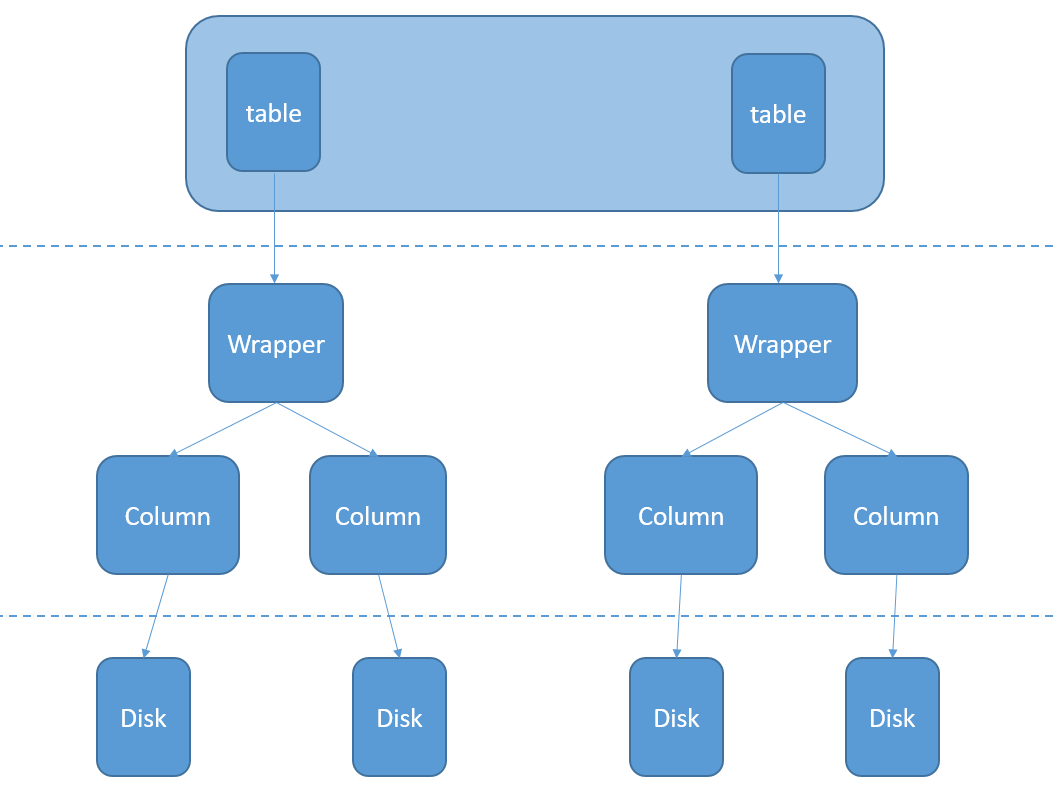
\includegraphics[width=1.0\linewidth]{cse291-1.png}\\
\subsection{connection APIs}
In the first layer we provide APIs to users. It include create table, append data, delete a key, select, and join tables.\\
In the wrapper we provide APIs to the database, the database can use append/delete to modify data in specific columns, get the whole data of one column and find the recent update of a key on one column.\\
In the column, we provide APIs to wrapper. Since there is one column manage for one column. We do not need to specify the column name. We just do get, edit by key, get all the data.\\
In the last column, we provide only two APIs: save file, and get file.\\


\section{Implementation of Action}
In this section we are going to explain how we implement those action required.
\subsection{append, edit, delete data}
For append and edit action, we use "set" to do this function. the set function take the table number and the key number to identify, plus a dictionary to indicate that which column does user want to set. Consider there is a table 1 and the column is name and birthday. And we want to set the name to "aa". What we do here is use the set function: set(1,key,{"name": "aa"}). The difference of append and edit is the completeness. In the edit function, the user can update only part of the column. Since we use column-based storage, the columns are stored separately. And it is reasonable to allow the user to update only part columns. However, the append is different. We need to make sure that every column contains all keys so we can maintain the consistency. So if the user want to append a record, we suggest it give us the values of all columns. If they do not do it, we will set the default value as an empty string. And for the delete action, obviously we need to delete the key in all columns. So there is no need the user indicate the columns, the database will set the value of every column to the None. To notice that, there is a difference between None and empty string. The empty string
\subsection{select, join, where}
For the select and join action, we need to scan all the table. At first, we think about that for every select/join we need to shuffle the storage, which means doing compaction and update every key to the newest. But later we find that necessary. We can join or select on records from old to new, in this way, the data maintain in order and we can let the new table to take care about the  compaction problem. In total, the join action is to join the record, not the special data. Let see if there are two tables: table A and table B. What we do is to take the table A and get all record. For every record, we find if the key is in the table B, if it is, we extract all data of that key and just put the record in the new database. And there is why we need to add record to all column, that is because we need to check the key to see if it is in the database. We do not have the global key, we can only pick up one column and do the check. And the select action is the same. We select the record rather that the true data. We never do the data shuffle and compaction ourselves. Only the disk manage determine the time of compaction. As for the where function, since we do not have the time to implement query engine. So the where is implemented as a function and it only support choose on keys.
\subsection{store in the memory}
The store in memory has nothing to do with the database management. After the column management, the memory store only need to deal with the bunch of key-value pairs. So we do this kind of things: if the value is None and the key has already in the map, we delete the key, if not, we add the None as record. The other things, we just add the record to the map. Once the size of the map is large enough, we pack the map and move it to an immutable table, and we make the map empty. Here is the difference between bigtable and the levelDB. The bigtable pack the memory cache and store them in the disk as some small file and use the minor compaction to merge them. The levelDB introduce the immutable table. This immutable table is in the memory and can only be read. So it only provide the search convinience. My best guess is that LevelDB focus on the performance but the bigtable consider about the scale problem. Bigtable uses all memory as cache so it can achieve better performance on frequent modification. Anyway, we use the idea of immutable table here so we can have better performance when select and join.


\subsection{compaction}
There are two types of compaction: \textbf{Minor compaction}, and \textbf{Major compaction}.

\begin{itemize}
  \item Minor compaction. The mechanism is similar to the "minor compaction" of LevelDB on SSTable level 0. Data to be compacted comes from the immutable table in memory. When the immutable becomes too large (in our implementation, this is managed by the first layer), it is completely dumped to disk, and emptied later.

  Data(key-value pairs) in immutable is sorted by key, and then written to file pair by pair. This is implemented by simply iterating all key-value pairs, and store them into an opened file.

  \item Major compaction. Major compaction is performed when there are too many minor compaction files. If the number of minor compaction exceeds $max_minor = 10$, those minor compactions files are all merged into a major compaction file.  Since all the key-value pairs are sorted, we can simply perform a merge join in those minor files. The merging process are described below.

  We use a priority queue to maintain the key that a pointer is pointing to. One after another, we get the smallest key from the queue, and if there are multiple keys that are smallest, then we keep the one from the newest minor compaction, and discard the others. Then we move those pointers to the next key-value pair in the file it points to. If there is a tombstone on that key, we will again discard it. Finally, this key is added to the array of contents of the major compaction. Keys in the content still obtain correct order.

  After merging, we simply write this major compaction to disk.

\end{itemize}

\subsection{bloom filter}

For each file, either it is a major compaction or it is a minor compaction, they will all have their own bloom filter to accelerate lookup. Bloomfilter is implemented with a large bit array, and several irrelated hash functions. When inserting, different hash functions will set some bits to true, and when testing whether a key exists, if all of the bits that this key mapped to are set, then it will return a true indicating this key might have exists in the set.\\

For our implementation, each table has maximum capacity of $1000$ keys, so the filter have $3500$ bits to ensure its probability of correctness.

\subsection{compression}
  Our implementation supports \textbf{dict-based compression}, and \textbf{general compression}. They can both be applied to a table to be stored and a table that is already stored. They can be both applied to the same table, as long as the configuration of the table, "gzip_compression" or "dict_compression", are set to $True$.

  \begin{itemize}
    \item \textbf{Dict-based compression}. In disk-based compression, the whole table will be scanned, and values are counted by its number of occurance. Then we construct Huffman tree by the counts of values, and replace each value with its huffman encoding.

    After values are encoded, when saving files, we simply replace the original value with the encoded value, and save it into disk one after another. The file still consists of key-value pairs, but the value now becomes the Huffman encoding of the original value.

    \item \textbf{General compression}. This is implemented using the built-in \textit{gzip} compression. Whenever needed, the original file will be read again, and compressed with the python \textit{gzip} library, and saved to disk. The original file can be kept, if the configuration does not allow to delete the original file.

  \end{itemize}

\subsection{store on the disk}
  All the data: the bloom filter, the key index, the dict-based compression dictionary, are stored on seperate files on the disk. Each table, or, to say, compaction, have its own data stored in its own file.\\

  \textbf{Saving compaction:}\\

  First, a bloom filter of this table is constructed for all the keys in this table. Then it will be written in its own file, named by table number and "\_bloom" suffix. Then the filter is dumped to file by python \textit{pickle} library, thus relieved us from the trival work to dump and load object from file. When it comes to table data and key index, we still use this library to dump them.

  Then, configuration of this table is examined. If the "dict\_compression" is set, we first construct the huffman encoding dictionary of the keys in this table, and store this table in a file ending with "\_comp\_dict" suffix. And then we replace the values in this table with its huffman encoded value.

  If "dict\_compression" is not set, or if the dict-based compression is completed, we dump the key-value pair in this table one by one. When writing objects, we also record the position that this pair is stored in this file, so that later on we can load it faster without loading the whole file. The data file has a suffix of "\_data".

  After writing data, we have the relative position of all the key-value pairs in the file it stored. At the same time, we also have the keys themselves. So we create a key index file with keys in the original data table as key, and position this record was written as value. This map is stored in the file with suffix "\_keys".\\

  \textbf{Loading compaction:}\\

  All the files, dict-based compression dictionary, key index table are loaded before loading the actual data. If the file is compressed by general compression, the data file will be decompressed first. If dict-based compression is enabled, the compression dictionary will be read before decompressing the data file.

  We also support fast loading, which is to load a key-value pair by key in any file. Since we have the relative position of all the key-value pairs, load by key only requires the relative position, the value, in the key index file. Thus we don't have to load the entire file when we only need several record with some specific keys.


\section{Test}
We run single case which cover most part of the database. Here is the idea of this test: create two tables, then select and join.
It is very simple idea but I think I have used every corner of this database.
The result is shown below:
The create table takes very little time, which is 1 us. And adding data to the table takes 0.025ms for 256 tuple. The select action takes also 0.026 ms. But the join takes a lot of time, the join takes 0.467 ms for those two tables.
\end{document}
